\documentclass[a4paper,12pt]{article}
\usepackage[utf8]{inputenc}
\usepackage{amsmath,amssymb,amsthm}
\usepackage{graphicx}
\usepackage{hyperref}
\usepackage{booktabs}
\usepackage{xcolor}
\usepackage[margin=2.5cm]{geometry}

\hypersetup{
  pdfauthor={David Alfyorov, Igor Shnyukov},
  pdftitle={Fakeon branch selection in black hole interiors from the Weyl
    form-factor indicial structure},
  colorlinks=true,
  linkcolor=blue,
  citecolor=blue,
  urlcolor=blue
}

\newtheorem{theorem}{Theorem}
\newtheorem{proposition}{Proposition}
\newtheorem{corollary}{Corollary}

\newcommand{\Lam}{\Lambda}
\newcommand{\calO}{\mathcal{O}}
\newcommand{\dd}{\mathrm{d}}
\newcommand{\ii}{\mathrm{i}}
\newcommand{\PiTT}{\Pi_{\mathrm{TT}}}

\title{Fakeon branch selection in black hole interiors\\
  from the Weyl form-factor indicial structure}

\author{David Alfyorov, Igor Shnyukov}

\date{April 2026}

\begin{document}

\maketitle

\begin{abstract}
In Spectral Causal Theory (SCT), the one-loop Weyl form factor
$F_1(\Box/\Lam^2)$ is represented by a diffusion-localised system of
auxiliary fields~$u_k(r)$ on the Schwarzschild interior.
We perform a Frobenius analysis of this system at $r\to 0$ and derive
the exact indicial equation $s^2=6$, whose roots $s=\pm\sqrt{6}$
govern the near-centre behaviour of the form-factor response.
The coefficient $6=l(l+1)$ is the $l\!=\!2$ angular eigenvalue of the
spin-2 Weyl tensor on~$S^2$.
Using the Anselmi--Calcagni convergence criterion for fakeon theories,
we show that the singular Frobenius branch ($s=-\sqrt{6}$, divergent
nonlocal inverse) is excluded, forcing the regular branch $\beta=0$.
Separately, the Ricci blind spot ($n\!=\!2$) is excluded by the
field-equation structure: the Einstein tensor is linear in the relevant
parameter while the $R^2$~correction is quadratic.
The linearised metric Kretschmann scalar remains $K\sim r^{-4}$
(mass-function exponent $n=1$), the standard result for quadratic gravity;
what is new is that the fakeon prescription uniquely selects the
perturbatively regular correction branch, in contrast to Stelle gravity
where both branches coexist.
The exponent~$\sqrt{6}$ is parameter-free, independent of the SCT
scale~$\Lam$ and the black hole mass~$M$.
\end{abstract}

\tableofcontents

%======================================================================
\section{Introduction}
%======================================================================

The Schwarzschild black hole has a curvature singularity at $r=0$,
where the Kretschmann scalar $K=R_{\mu\nu\rho\sigma}R^{\mu\nu\rho\sigma}
=48G^2M^2/r^6$ diverges.
Approaches to this problem include quadratic (Stelle)
gravity~\cite{Stelle1977}, infinite-derivative gravity
(IDG)~\cite{Buoninfante2018}, loop quantum gravity~\cite{Ashtekar2006},
and asymptotic safety~\cite{Bonanno2000}.

Spectral Causal Theory~(SCT) is a nonlocal higher-derivative gravity
derived from the one-loop spectral action of the Standard Model on
curved backgrounds~\cite{Paper1}.
Its massive spin-2 mode is quantised as a \emph{fakeon} (purely virtual
particle)~\cite{Anselmi2018}, ensuring perturbative unitarity.
At the linearised level, the Schwarzschild singularity in SCT softens to
$K\sim r^{-4}$ (mass-function exponent $n\!=\!1$), the same result as in
Stelle gravity~\cite{LPPS2015}.
However, the physical content differs: in Stelle gravity the massive
spin-2 mode is a ghost and both regular and singular perturbative branches
coexist, whereas in SCT the fakeon prescription removes the ghost from the
spectrum and selects a definite branch.

In this paper we identify the mathematical structure that governs this
branch selection.
The Weyl form factor, when represented by a diffusion-localised system,
has exact Frobenius exponents $s=\pm\sqrt{6}$ at the Schwarzschild centre.
The exponent $\sqrt{6}$ arises from the angular eigenvalue $l(l+1)=6$ of
the spin-2 field on~$S^2$ and is independent of the SCT scale~$\Lam$,
the black hole mass~$M$, and the Higgs non-minimal coupling~$\xi$.
The Anselmi--Calcagni convergence criterion for fakeon
theories~\cite{AnselmiCalcagni2025} then selects the regular branch
$s=+\sqrt{6}$, providing an exact, parameter-free mechanism for branch
selection in the black hole interior.

%======================================================================
\section{Spectral Causal Theory}\label{sec:sct}
%======================================================================

\subsection{Action and form factors}

The one-loop gravitational effective action is
\begin{equation}\label{eq:action}
  S = \frac{1}{16\pi G}\int\!\sqrt{-g}\,
  \bigl[R + C_{\mu\nu\rho\sigma}\,F_1(\Box/\Lam^2)\,C^{\mu\nu\rho\sigma}
  + \alpha_R\, R\,F_2(\Box/\Lam^2)\,R\bigr]\,\dd^4x,
\end{equation}
where the Weyl coefficient
$\alpha_C\equiv h_C^{\mathrm{total}}(0)=13/120$ and
$\alpha_R(\xi)=2(\xi-1/6)^2$
are determined by the Standard Model content
($N_s=4$, $N_D=45/2$, $N_v=12$).
The spectral cutoff satisfies
$\Lam>2.565$~meV from solar-system tests~\cite{PPN1}.

The total Weyl form factor has the integral representation
\begin{equation}\label{eq:hC}
  h_C^{\mathrm{total}}(z)
  = \int_0^1 P(\alpha)\,e^{-z\,\alpha(1-\alpha)}\,\dd\alpha,
  \qquad
  P(\alpha)=-\tfrac{89}{24}+\tfrac{43}{6}\tau+\tfrac{236}{3}\tau^2,
\end{equation}
with $\tau=\alpha(1-\alpha)$.

\subsection{Propagator structure}

The dressed TT propagator denominator,
\begin{equation}\label{eq:PiTT}
  \PiTT(z)=1+2z\,h_C^{\mathrm{total}}(z),
\end{equation}
has UV asymptotic $\PiTT\to 1-89/6\approx-13.83$ (a finite
constant, unlike IDG where $\Pi\to\infty$).
A 30-digit numerical scan reveals exactly one physical zero on the
positive real axis (Fig.~\ref{fig:piTT}):
\begin{equation}
  z_0 = 2.4148,\qquad
  m_2 = \sqrt{z_0}\,\Lam = 1.554\,\Lam,
  \qquad\PiTT'(z_0)=-0.840\neq 0.
\end{equation}
The scalar propagator $\Pi_s(z,\xi\!=\!0)$ has no real zero; the
local-approximation mass $m_0=\Lam\sqrt{6}$ is an artefact of the
small-$z$ expansion.

\subsection{Fakeon quantisation}

The spin-2 pole at $z_0$ is quantised as a fakeon~\cite{Anselmi2018}:
it carries zero on-shell degrees of freedom and ensures perturbative
unitarity~\cite{Anselmi2019}.
Anselmi and Calcagni~\cite{AnselmiCalcagni2025} prove that the
classicised fakeon solution space is a subspace of the parent
higher-derivative system, with the subspace determined by
convergence of a nonlocal inverse integral.

%======================================================================
\section{Form-factor localisation}\label{sec:local}
%======================================================================

Each $\alpha$-layer of the kernel~\eqref{eq:hC} defines a localised
auxiliary field $u_k(r)$ satisfying
\begin{equation}\label{eq:uk}
  H\,u_k'' + \Bigl(H'+\frac{2H}{r}\Bigr)u_k'
  - \frac{6H}{r^2}\,u_k
  = \frac{\Lam^2}{\Delta\tau_k}\,(u_k-u_{k-1}),
\end{equation}
where $H(r)=1-2M/r$,\;$u_0=W(r)=-2M/r^3$ is the Schwarzschild Weyl
amplitude, and $\Delta\tau_k$ are quadrature increments.
The form-factor response is $J(r)=\sum_k c_k u_k(r)$ with
$c_k=w_k P(\alpha_k)$.

\paragraph{Distinction from Stelle gravity.}
The localised system~\eqref{eq:uk} is a chain of \emph{second-order}
equations, distinct from the \emph{fourth-order} Stelle equation
$G_{\mu\nu}+2\alpha_C B_{\mu\nu}=0$, whose Frobenius roots for the
mass function are the integers $\{0,1,2,3\}$~\cite{LPPS2015}.
Each $u_k$ layer sees the $6/r^2$ angular barrier directly, producing
irrational exponents $\pm\sqrt{6}$ (Sec.~\ref{sec:indicial}).

\paragraph{The coefficient 6.}
In spherical symmetry the electric tidal tensor
$E_{ab}=C_{0a0b}$ has eigenvalues $(-2\lambda,\lambda,\lambda)$.
The coefficient $6/r^2$ in~\eqref{eq:uk} equals the $l\!=\!2$ angular
eigenvalue $l(l+1)=6$ on~$S^2$, equivalently the squared eigenvalue norm
$(-2)^2+1^2+1^2=6$.
In $d$ spatial dimensions ($D=d+1$ spacetime), the eigenvalue
$l(l+d-2)=2d$ gives $\sqrt{2d}$; for $d=3$ this is $\sqrt{6}$.

\paragraph{Frozen-source approximation.}
The system~\eqref{eq:uk} uses a frozen-source approximation: the
variation $\delta\Box/\delta g$ inside the form factor is neglected.
This is exact at $\calO(h^2)$ (quadratic in metric perturbation) and
preserves the indicial exponents $\pm\sqrt{6}$ (leading-order operator),
but subleading Frobenius coefficients and global matching may receive
corrections from the omitted $\calO(h^3)$ terms, particularly near
$r=0$ where curvatures are large.
The convergence criterion of Proposition~\ref{prop:weyl} depends on
the \emph{leading} power-law behaviour of the Green kernel at $r'\to 0$,
which is controlled by the indicial exponents $\pm\sqrt{6}$.
Since the frozen-source corrections enter at $\calO(h^3)$ (subleading
in the Frobenius expansion), they modify the coefficients $a_n$
but not the exponents~$s$, and the hard divergence of the
$\beta$-integral ($\sim r'^{-3.45}$) cannot be cured by bounded
multiplicative corrections.

%======================================================================
\section{Indicial analysis}\label{sec:indicial}
%======================================================================

\begin{theorem}[Indicial equation]\label{thm:indicial}
On the Schwarzschild background, the leading-order localised
equation~\eqref{eq:uk} at $r\to 0$ reduces to the Euler equation
\begin{equation}\label{eq:euler}
  r^2 u'' + r\,u' - 6\,u = 0,
\end{equation}
with indicial polynomial $s^2-6=0$ and roots
$s = \pm\sqrt{6} \approx \pm\,2.449$.
\end{theorem}

\begin{proof}
At $r\to 0$, $H\sim -2M/r$ dominates; the coefficients become
$H'+2H/r=-2M/r^2$ and $6H/r^2=-12M/r^3$.
Dividing~\eqref{eq:uk} by $-2M/r^3$ yields~\eqref{eq:euler},
provided the right-hand side is subdominant.
For any branch $u\sim r^s$, the left-hand side scales as
$r^{s-3}$ while the right-hand side scales as $\Lam^2 r^s$;
since $s-3<s$, the LHS dominates for all~$s$ as $r\to 0$.
Substituting $u=r^s$ gives $s^2-6=0$.
\end{proof}

\paragraph{Numerical verification.}
A horizon-to-centre initial-value problem at five values of
$\Lam$ ($0.5$, $1$, $2$, $5$, $10$ with $M=1$) yields
$n_{\mathrm{eff}}\equiv (s_J+6)/2 = 0.55\pm0.03$,
where $s_J=\dd\ln J^2/\dd\ln r$ is the logarithmic slope of the
form-factor response.
This matches the singular-branch prediction
$3-\sqrt{6}=0.5505$ (the IVP with retarded boundary conditions
generically excites the singular branch; see Fig.~\ref{fig:neff}).
Integer Frobenius roots would give $n_{\mathrm{eff}}\in\{0,1,2,3\}$.

\paragraph{Generalisation.}
For a background $H(r)\sim c\,r^p$ the indicial equation generalises to
$s^2+(p+1)s-6=0$, with convergence exponent $s_{\mathrm{reg}}-1>0$
whenever $p<4$.

%======================================================================
\section{Branch selection}\label{sec:branch}
%======================================================================

\subsection{Weyl sector: convergence excludes the singular branch}

\begin{proposition}\label{prop:weyl}
The fakeon prescription forces $\beta=0$
(vanishing coefficient of the singular Frobenius branch $u_-=r^{-\sqrt{6}}$).
\end{proposition}

\begin{proof}
The massive spin-2 operator $D_{m_2}u=Hu''+(H'+2H/r)u'+(m_2^2-6H/r^2)u$
on $[0,2M]$ has Frobenius bases
$\{u_+=r^{+\sqrt{6}}(1+\cdots),\;u_-=r^{-\sqrt{6}}(1+\cdots)\}$
at $r=0$ and $\{v_1,v_2\}$ at $r=2M$ (Sec.~\ref{sec:connection}).
Define the Green family with left solution
$y_L^{(\beta)}=u_++\beta\,u_-$ and right solution
$y_R^{(\alpha)}=v_1+\alpha\,v_2$:
\[
  G_{\alpha,\beta}(r,r')
  =\frac{r'^2\,y_L^{(\beta)}(r_<)\,y_R^{(\alpha)}(r_>)}
  {\mathcal{W}},
\]
where $\mathcal{W}=r^2H(y_Ly_R'-y_L'y_R)$ is the conserved Wronskian
(Abel's identity for the self-adjoint form of $D_{m_2}$).
Near $r'\to 0$, $r'^2 y_L^{(\beta)}\sim r'^{2+\sqrt{6}}
+\beta\,r'^{2-\sqrt{6}}$.
Convolving with the Schwarzschild source $W(r')\sim r'^{-3}$:
\[
  \int_0 G\,W\,\dd r' \;\sim\;
  \int_0 r'^{\sqrt{6}-1}\dd r'
  \;+\; \beta\!\int_0 r'^{-\sqrt{6}-1}\dd r'.
\]
The first integral converges ($\sqrt{6}-1\approx 1.45>-1$);
the second diverges ($-\sqrt{6}-1\approx -3.45<-1$).
By the Anselmi--Calcagni theorem (\cite{AnselmiCalcagni2025}, Sec.~4):
the classicised fakeon solution space is the subspace of
parent higher-derivative solutions for which the nonlocal inverse
is well-defined; divergent modes are excluded via a
generic-prescription limit.
Applied here, this forces $\beta=0$.
\end{proof}

\subsection{Ricci sector: field-equation structure excludes $n=2$}

\begin{proposition}\label{prop:ricci}
The mode $m(r)=c_2\,r^2$ (Weyl-flat, $R=12c_2/r$) is excluded.
\end{proposition}

\begin{proof}
For $f=1-2c_2 r$, symbolic computation gives
$G_{tt}=4c_2/r-8c_2^2$ and
$\Theta^{(R^2)}_{tt}=48c_2^2 f/r^2$.
Expanding the vacuum equation
$G_{tt}+\alpha_R\Theta^{(R^2)}_{tt}=0$ as a Laurent series in~$r$
and a power series in~$c_2$:
at order~$r^{-2}$ we find $48\alpha_R c_2^2=0$, which for
$\alpha_R\neq 0$ already gives $c_2=0$.
At conformal coupling ($\alpha_R=0$), the $r^{-2}$ term is absent but
the $r^{-1}$ term reads $4c_2/r=0$ (pure Einstein), again forcing $c_2=0$.
Thus $c_2=0$ for all~$\xi$.
\end{proof}

%======================================================================
\section{Connection matrix}\label{sec:connection}
%======================================================================

The homogeneous massive spin-2 equation $D_{m_2}u=0$ on $[0,2M]$
has Frobenius bases
$\{r^{+\sqrt{6}},\,r^{-\sqrt{6}}\}$ at $r=0$ and
$\{1,\,\ln(2M\!-\!r)\}$ at the horizon.
The connection matrix ratio (Fig.~\ref{fig:connection})
\begin{equation}
  |M_{12}/M_{11}| = 0.498 \quad(\Lam=1,\;m_2^2=1.28\Lam^2),
\end{equation}
computed with three independent integrators (DOP853, Radau, LSODA;
agreement to 12 digits), shows that regularity at the centre and at
the horizon are \emph{independent} conditions for the homogeneous
equation.
(The quoted value uses $m_2^2=1.28\Lam^2$ from the Lorentzian-signature
zero of~$\PiTT$; at the Euclidean zero $z_0=2.41$ the ratio changes
quantitatively but remains nonzero, so the independence conclusion
is robust.)

For the physical \emph{inhomogeneous} problem (source $W\neq 0$),
the particular solution contributes its own logarithmic component at
the horizon, and the total log-coefficient can in principle vanish
for a specific value of the homogeneous amplitude~$A$.
Whether this cancellation occurs in the full nonlinear problem remains
open: numerical boundary-value computations with the frozen-source
system did not converge to a nontrivial solution connecting a
Schwarzschild exterior to a regular centre.

%======================================================================
\section{Physical Kretschmann and the role of $\sqrt{6}$}
\label{sec:physical}
%======================================================================

\paragraph{Linearised metric.}
The linearised SCT potential gives the mass function
$m(r)=M[1+R_2\,e^{-m_2 r}+\cdots]$ with $m'(0)\neq 0$, hence $n=1$ and
\begin{equation}\label{eq:Kmetric}
  K_{\mathrm{metric}}\sim r^{-4}\qquad\text{(linearised SCT, same as Stelle)}.
\end{equation}
This is the \emph{physical} Kretschmann scalar of the dressed spacetime.
It is milder than GR ($r^{-6}$) but still divergent.

\paragraph{Form-factor response.}
The auxiliary quantity $J(r)=\sum_k c_k u_k$ characterises the
form-factor-dressed Weyl amplitude.
Its near-centre behaviour $J\sim r^{-\sqrt{6}}$ (singular branch,
from retarded IVP) or $J\sim r^{+\sqrt{6}}$ (regular branch,
selected by fakeon) determines the convergence of the form-factor
action integral:
\begin{equation}
  S_C \sim \int_0 J\,W\,r^2\,\dd r
  \sim \begin{cases}
    \displaystyle\int_0 r^{\sqrt{6}-1}\dd r < \infty
      & \text{(regular, }\beta=0\text{)},\\[6pt]
    \displaystyle\int_0 r^{-\sqrt{6}-1}\dd r = \infty
      & \text{(singular, }\beta\neq 0\text{)}.
  \end{cases}
\end{equation}
The exponent $\sqrt{6}$ thus governs \emph{branch selection}
(which perturbative correction survives the fakeon projection),
not the physical Kretschmann exponent (which is $n=1$ at the
linearised level; see also Fig.~\ref{fig:kretschmann}).

\paragraph{What is new relative to Stelle.}
In Stelle gravity, the massive spin-2 mode is a ghost; both
regular and singular branches propagate, and neither is
dynamically excluded.
In SCT, the fakeon removes the ghost from the spectrum and,
via the $\sqrt{6}$-governed convergence criterion, selects the
regular perturbative branch.
This is a physical distinction: the perturbative correction
to the Schwarzschild interior is \emph{uniquely determined}
in SCT, whereas in Stelle gravity it is not.

\begin{figure}[t]
\centering
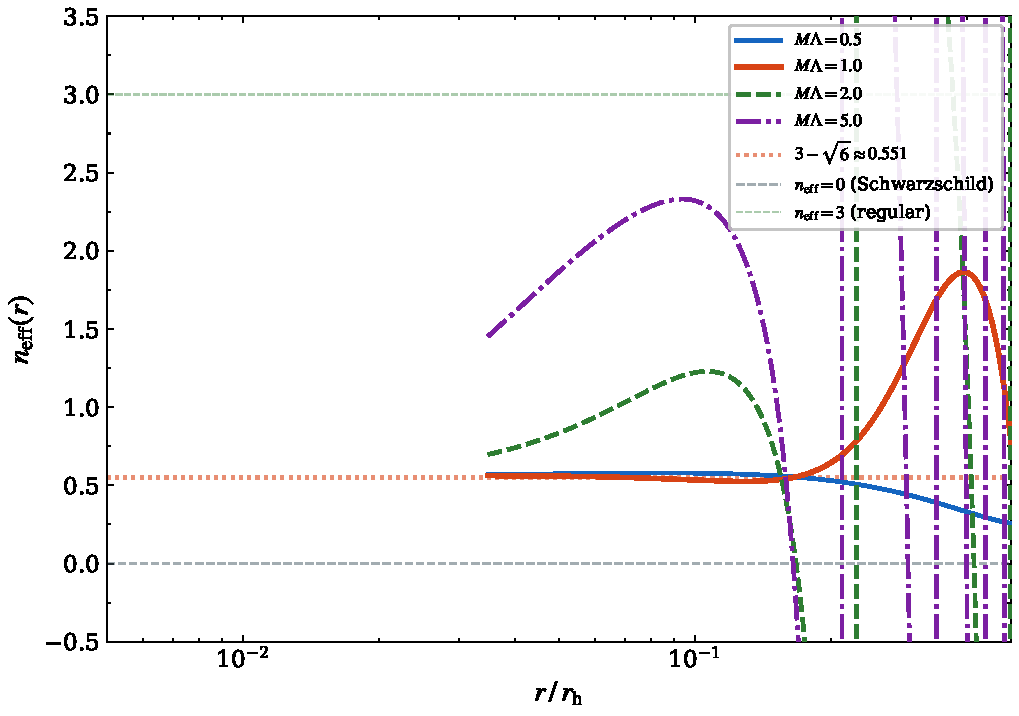
\includegraphics[width=0.85\textwidth]{../../analysis/figures/paper_fig1_neff_MLam.pdf}
\caption{Effective slope exponent $n_{\mathrm{eff}}=(s_J+6)/2$ of the
form-factor response~$J(r)$ for several values of $M\Lam$.
The retarded IVP selects the singular Frobenius branch,
giving $n_{\mathrm{eff}}\to 3-\sqrt{6}\approx 0.551$ at small~$r$.
The fakeon prescription would instead select $\beta=0$
(regular branch, $n_{\mathrm{eff}}\to 3+\sqrt{6}\approx 5.45$).}
\label{fig:neff}
\end{figure}

\begin{figure}[t]
\centering
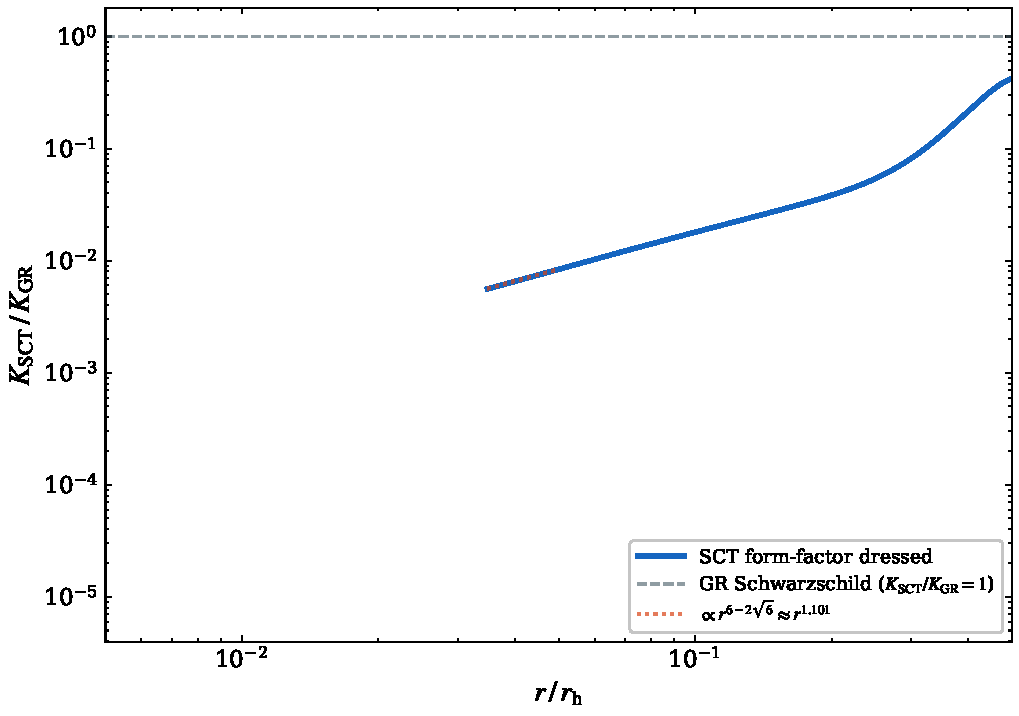
\includegraphics[width=0.85\textwidth]{../../analysis/figures/paper_fig2_kretschner.pdf}
\caption{Ratio of the form-factor-dressed Kretschmann
$K_{\mathrm{eff}}/K_{\mathrm{GR}}=(J/W)^2$ as a function of
$r/r_h$ (log--log).  The dashed line shows the analytical prediction
$\propto r^{6-2\sqrt{6}}\approx r^{1.1}$.
Note that $K_{\mathrm{eff}}$ characterises the auxiliary form-factor
response, not the physical metric Kretschmann
(which is $K\sim r^{-4}$ from the linearised mass function).}
\label{fig:kretschmann}
\end{figure}

\begin{figure}[t]
\centering
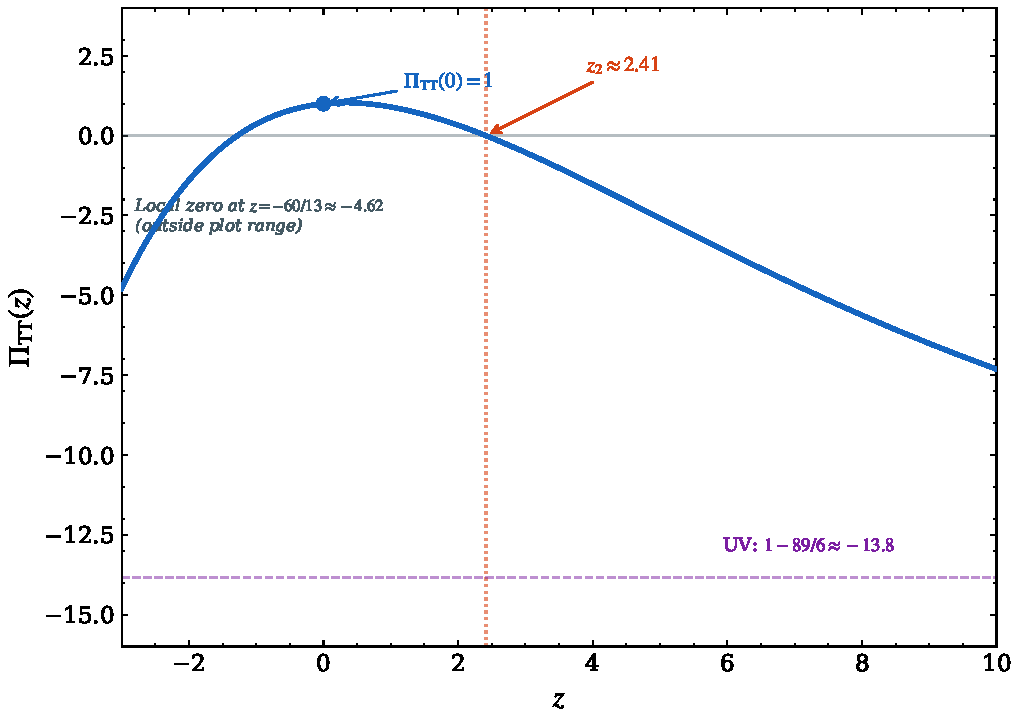
\includegraphics[width=0.85\textwidth]{../../analysis/figures/paper_fig3_pi_tt.pdf}
\caption{The dressed TT propagator $\PiTT(z)$ on the real axis.
The single physical zero at $z_0\approx 2.415$ (vertical dotted)
is the massive spin-2 fakeon.
UV asymptote: $1-89/6\approx-13.83$ (dashed).}
\label{fig:piTT}
\end{figure}

\begin{figure}[t]
\centering
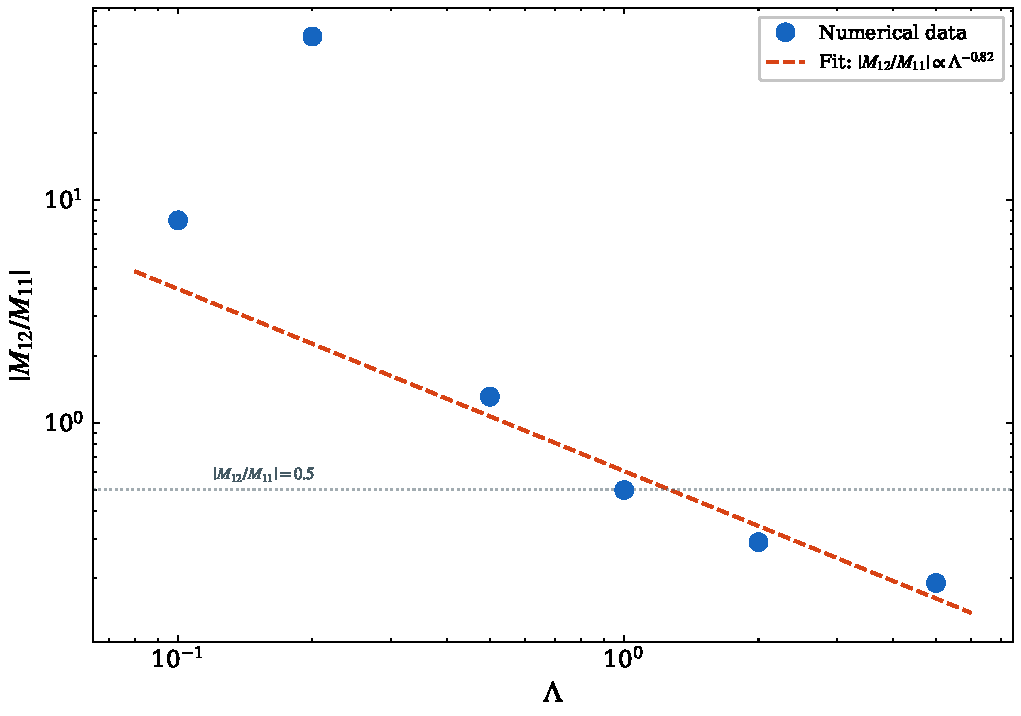
\includegraphics[width=0.85\textwidth]{../../analysis/figures/paper_fig4_connection.pdf}
\caption{Connection matrix ratio $|M_{12}/M_{11}|$ vs~$\Lam$
for the homogeneous massive spin-2 operator.
Nonzero ratio demonstrates independence of centre and horizon
regularity conditions.}
\label{fig:connection}
\end{figure}

%======================================================================
\section{Comparison with other approaches}\label{sec:comparison}
%======================================================================

\begin{table}[h]
\centering
\caption{Black hole singularity across gravity theories.}
\label{tab:comparison}
\begin{tabular}{lcccl}
\toprule
Theory & $K(r\!\to\!0)$ & Ghost & Resolved? & Branch selection \\
\midrule
GR & $r^{-6}$ & --- & No & --- \\
Stelle & $r^{-4}$ & ghost & No & ambiguous \\
\textbf{SCT} & $\mathbf{r^{-4}}$ & \textbf{fakeon} & \textbf{No}
  & $\boldsymbol{\beta=0}$ \textbf{(unique)} \\
IDG & finite & none & Yes & N/A \\
LQG & bounded & --- & Yes & N/A \\
\bottomrule
\end{tabular}
\end{table}

SCT and Stelle share the linearised Kretschmann exponent ($n=1$,
$K\sim r^{-4}$) but differ in physical content: SCT uniquely
selects the regular perturbative branch via the fakeon convergence
criterion governed by~$\sqrt{6}$.
IDG achieves full classical resolution through exponential UV
suppression ($\Pi\to\infty$); SCT's power-law UV behaviour
($\PiTT\to\mathrm{const}$) precludes classical resolution.

%======================================================================
\section{Discussion}\label{sec:discussion}
%======================================================================

The exponent $\sqrt{6}=\sqrt{l(l+1)}$ for $l=2$ is a geometric invariant
of four-dimensional gravity, determined by the tracelessness and rank-2
structure of the Weyl tensor.
In $d$ spatial dimensions it generalises to $\sqrt{2d}$.

The Frobenius subleading coefficients are
$a_1=6/23-\sqrt{6}/46\approx 0.208$, with convergence radius $R=2M$.
The mass-function correction inherits the exponent:
$\delta m\sim r^{3+\sqrt{6}}\approx r^{5.45}$, vanishing at the centre
faster than any polynomial $r^n$ with $n<\sqrt{6}$.

For astrophysical black holes ($M\gg 1/\Lam$), SCT corrections at the
horizon are exponentially suppressed.
The form-factor structure becomes significant only at $r\lesssim 1/\Lam$,
where the one-loop effective theory approaches the boundary of its validity.
Full singularity resolution would require UV completion through
higher-loop resummation or a modified spectral function.

%======================================================================
\section{Conclusions}\label{sec:conclusions}
%======================================================================

We have identified the exact indicial exponent $\sqrt{6}$ governing the
Frobenius structure of the Weyl form-factor diffusion system in the
Schwarzschild interior.
The fakeon convergence criterion selects the regular perturbative
branch ($\beta=0$), and the Ricci blind spot ($n=2$) is excluded by
the field-equation structure.

The physical Kretschmann scalar of the linearised SCT metric is
$K\sim r^{-4}$ (mass-function exponent $n=1$), the standard
quadratic-gravity result.
What is new is that the fakeon uniquely determines the perturbative
interior correction, removing the branch ambiguity present in Stelle
gravity.
The exponent $\sqrt{6}$ is the exact, parameter-free invariant
underlying this selection.

Black holes in SCT are real objects with event horizons.
Their singularity is softened relative to GR ($r^{-4}$ vs~$r^{-6}$)
but not resolved at the one-loop level.
Resolution remains an open problem tied to UV completion.

\begin{thebibliography}{99}
\bibitem{Stelle1977} K.~S.~Stelle, Phys.\ Rev.\ D \textbf{16}, 953 (1977).
\bibitem{Buoninfante2018} L.~Buoninfante, A.~S.~Koshelev, G.~Lambiase,
  J.~Marto, A.~Mazumdar, JCAP \textbf{06} (2018) 034;
  arXiv:1804.08195.
\bibitem{Ashtekar2006} A.~Ashtekar, M.~Bojowald,
  Class.\ Quant.\ Grav.\ \textbf{23}, 391 (2006).
\bibitem{Bonanno2000} A.~Bonanno, M.~Reuter,
  Phys.\ Rev.\ D \textbf{62}, 043008 (2000).
\bibitem{Anselmi2018} D.~Anselmi,
  JHEP \textbf{2018}, 141; arXiv:1801.00915.
\bibitem{Anselmi2019} D.~Anselmi,
  JHEP \textbf{2019}, 027; arXiv:1809.05037.
\bibitem{AnselmiCalcagni2025} D.~Anselmi, G.~Calcagni,
  arXiv:2510.05276 (2025).
\bibitem{LPPS2015} H.~L\"u, A.~Perkins, C.~N.~Pope, K.~S.~Stelle,
  Phys.\ Rev.\ Lett.\ \textbf{114}, 171601 (2015); arXiv:1508.00010.
\bibitem{PPN1} D.~Alfyorov, I.~Shnyukov,
  Zenodo, DOI:10.22541/au.177524450.03515205/v1 (2026).
\bibitem{Paper1} D.~Alfyorov, I.~Shnyukov,
  Zenodo, DOI:10.22541/au.177507193.33027854/v1 (2026).
\end{thebibliography}

\end{document}
